\documentclass[a4paper,11pt]{article}

\usepackage[left=20mm, text={170mm, 240mm}, top=30mm]{geometry}
\usepackage[czech]{babel}
\usepackage[IL2]{fontenc}
\usepackage[utf8x]{inputenc}
\usepackage{enumitem}
\usepackage{scrextend}
\usepackage{lscape}
\usepackage{times}
\usepackage{graphicx}
\usepackage[T1]{fontenc}
\usepackage{lmodern}
\usepackage{indentfirst}
\usepackage{pgfplots}
\usepackage{pgfplotstable}
\usepackage{mathtools}
\usepackage{amsfonts}
\usepackage{amsthm}
\usepackage{booktabs}
\usepackage{longtable}
\usepackage{tabto}

\setlength{\parskip}{1em}
\pgfplotsset{compat=1.15}

\pgfplotstableset{% global config, for example in the preamble
  every head row/.style={before row=\toprule,after row=\midrule},
  every last row/.style={after row=\bottomrule},
  fixed
}

\begin{document}

\begin{titlepage}

	\begin{center}
		
        
\includegraphics[width=4.1cm,keepaspectratio,trim={1.2cm 1.2cm 1.2cm 1.2cm},clip]{./template-fig/VUT_symbol_barevne_CMYK_CZ}%symbol VUT

		{\Huge\textsc{Vysoké učení technické v~Brně}}\\
		\medskip
		{\huge\textsc{Fakulta informačních technologií}}\\
		\vspace{\stretch{0.382}}
		{\huge 2. Hamiltonova cesta a cyklus v grafu}\\
		\medskip
		{\LARGE IAL - Algoritmy: Náhradní projekt - skupinový}\\
		\vspace{\stretch{0.618}}
	\end{center}

    \noindent xdrahn00@stud.fit.vutbr.cz\\ xvavri10@stud.fit.vutbr.cz \Large {\hfill Brno, \today}

\end{titlepage}

\section{Zadání}

Cestu v grafu, ve které se vyskytuje každý vrchol právě jednou, nazýváme Hamiltonovou cestou. Má-li tato cesta počátek a konec v jednom jediném vrcholu, pak se jedná o Hamiltonův cyklus v grafu. 

Vytvořte program pro hledání Hamiltonovy cesty (pro dva zadané vrcholy) a Hamiltonova cyklu v neorientovaném grafu. 

Pokud existuje více řešení, nalezněte všechna. Výsledky prezentujte vhodným způsobem. Součástí projektu bude načítání grafů ze souboru a vhodné testovací grafy. V dokumentaci uveďte teoretickou složitost úlohy a porovnejte ji s experimentálními výsledky.


\section{Úvod}

Dokumentace popisuje implementaci a návrh řešení k zadání č. 2 Hamiltonova cesta a cyklus v grafu (přesná kopie zadání se nachází výše).

\section{Vstupní podmínky}

V kontrolování předpokladů splnitelnosti je snaha předejít zbytečnému prohledávání grafu algoritmicky. Základní vstupní podmínky jsou v programu naimplementovány, rozšířené vstupní podmínky slouží pouze pro informaci při zapnutém `debug` přepínači. 

\subsection{Základní vstupní podmínky}

Není možné v grafu nalézt Hamiltonovu cestu a cyklus pokud nejsou splněna následující pravidla:
\begin{enumerate}
	\item Počet vrcholů v grafu musí být větší než 2
	\item Graf musí mít minimálně stupeň 1 pro každý vrchol pro nalezení Hamiltonovi cesty
    \item Graf musí mít pro každý vrchol minimálně stupeň 2 pro každý vrchol pro nalezení Hamiltonova cyklu
\end{enumerate}
\newpage
\subsection{Rozšířené vstupní podmínky}

K ověření zda lze v grafu nalézt Hamiltonovu cestu a cyklus stačí splnění některé z následujících podmínek. Nesplnění žádné z nich nutně nemusí znamenat, že graf Hamiltonovu cestu nebo cyklus neobsahuje.
\begin{enumerate}
    \item \textbf{Diracova} podmínka - každý vrchol má stupeň alespoň ½ celkového počtu vrcholů
    \item \textbf{Oreho} podmínka - každá dvojice vrcholů nespojených hranou má součet stupňů alespoň jako je celkový počet vrcholů
    \item \textbf{Pósova} - pro každé přirozené číslo k < ½ celkého počtu vrcholů existuje počet vrcholů, jejichž stupeň nepřevyšuje k, menší než k
\end{enumerate}

\section{Algoritmus - Brute force}

Algoritmus začíná prohledávat graf na počátečním vrcholu. Počáteční vrchol může být zadaný uživatelem. Algoritmus pro počáteční bod projde všechny jeho hrany a rekurzivně se zavolá pro vrcholy ke kterým jednotlivé hrany vedou. Nezavolá se rekurzivně a algoritmus pro konkrétní variantu cesty skončí neúspěchem pouze v případě pokud byl vrchol na této konkrétní variantě cesty již prozkoumán nebo při nalezení posledního vrcholu. Poslední vrchol může být také zadaný uživatelem. Bez uvedení vrcholů uživatelem se za první a cílový vrchol vybere vrchol uvedený na prvním řádku zdrojového grafu a hledá se tedy Hamiltonův cyklus. Tento algoritmus je dále označován jako Brute force, protože neobsahuje žádnou optimalizaci.

\section{Vstupní data}

Vstupní data jsou uloženy v souborech \textbf{.in}. Na každém řádku v tomto souboru se nachází právě dva názvy, které značí daný vrchol. Význam spojení dvou vrcholů značí to, že mají společnou hranu. Tento soubor je potom pomocí jednoduchého python skriptu převeden do formátu \textbf{.dot} (graph description language) a nakonec s pomocí knihovny Graphviz\cite{graphviz} i do formátu \textbf{.png}.

\newpage

\begin{figure}[!h]
\caption{Formát vstupních dat}
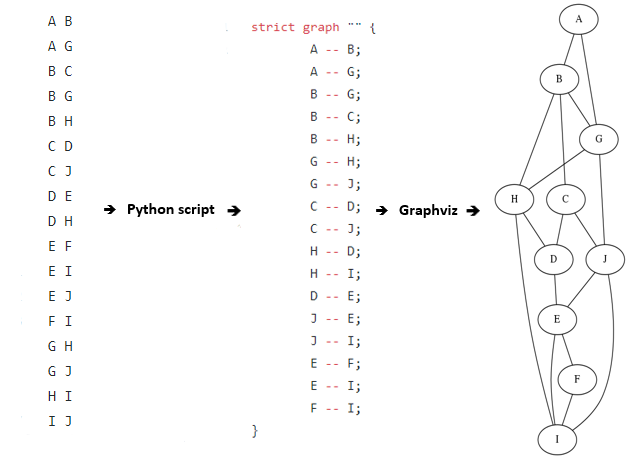
\includegraphics[width=4.1cm,keepaspectratio,trim={1.2cm 1.2cm 1.2cm 1.2cm},clip]{./inputData.png}
\centering
\end{figure}
\hspace{0,55cm}\textbf{\LARGE{.in}} \hspace{6cm} \textbf{\LARGE{.dot}} \hspace{4,6cm} \textbf{\LARGE{.png}}



\section{Teoretická složitost}

\subsection{Analýza}
\begin{itemize}
	\item Celkem existuje $(|V|-1)!$ kružnic
	\item Každá kružnice má $|V|$ hran
	\item Potřebujeme zpracovat $|V|$hran
	\item Časová složitost je faktoriálová - $O(n!)$
	\item Celkem existuje $(V-1)!/2$ řešení
	\item Předpokládáme rychlost zpracovávání 1 000 000 000 hran za sekundu
\end{itemize}

\newpage

\subsection{Výpočet}
\pgfplotstabletypeset[
font={\small},
begin table=\begin{longtable},
	columns/vertices/.style={column name=Vrcholy},
	columns/edges/.style={column name=Počet hran ke zpracování},
	columns/solutions/.style={column name=Počet řešení},
	columns/executed_time/.style={string type, column name=Čas zpracování},
	end table=\end{longtable},
]{./../complexity/theoretical_complexity.txt}
\section{Experimentální ověření složitosti}

K naměření dat byly použity grafy s počtem vrcholů od 3 do 13 uvedené ve složce `complexity/graphs`. Všechny tyto grafy obsahují hrany propojující každý vrchol se všemi ostatními. Vstupní parametry nejsou zadány, je hledaný Hamiltonův cyklus z $A$ do $A$. Počet nalezených cyklů odpovídá faktoriálu $(V - 1)!$ kde $V$ značí počet vrcholů.

\pgfplotstabletypeset[
  font={\small},
  begin table=\begin{longtable},
  columns/graph/.style={string type, column name=Graf},
  columns/vertices/.style={column name=Vrcholy},
  columns/edges/.style={column name=Hrany},
  columns/explored_vertices/.style={column name=Prozkoumané vrcholy},
  columns/executed_time/.style={column name=Čas [s]},
  columns/results/.style={column name=Výsledky},
  columns/allocs/.style={column name=Alokování},
  columns/allocated_memory/.style={column name=Alokovaná pamět [byte]},
  end table=\end{longtable},
]{./../complexity/brute_force_info.txt}

%\begin{figure}[!h]
%    \centering
%    \caption{Příklad grafu s 5-ti vrcholy obsahující hrany propojující každý vrchol se všemi ostatními}
%    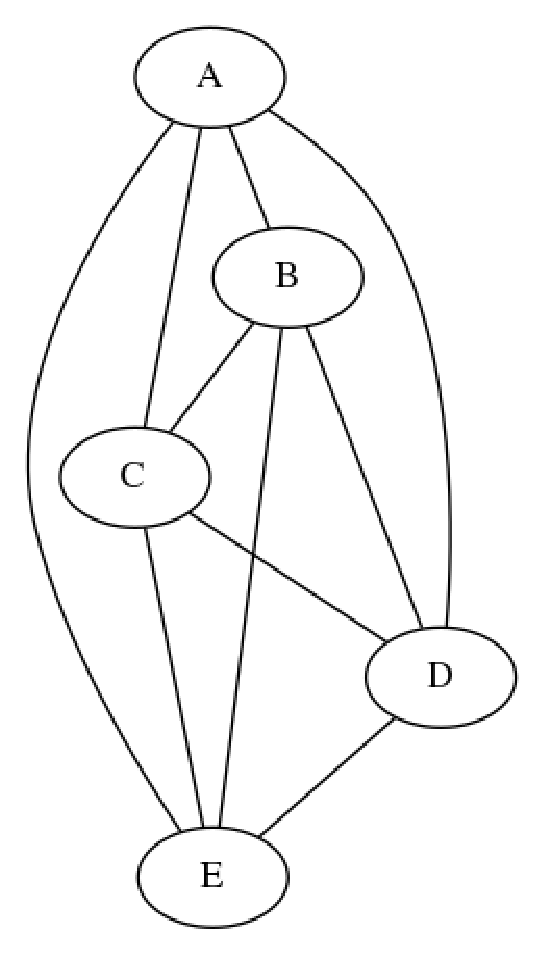
\includegraphics[width=0.2\textwidth]{./template-fig/5v}
%\end{figure}

\newpage
\subsection{Experimentální ověření prostorové složitosti}

\begin{figure}[h]
\centering
\begin{tikzpicture}
\begin{axis}[
    xlabel={Počet vrcholů grafu (hrany každý s každým)},
    ylabel={Velikost alokované paměti [byte]},
    legend pos=north west,
    legend entries={Algoritmus - Brute force},
]
\addplot table [x=vertices,y=allocated_memory] {./../complexity/brute_force_info.txt};
\end{axis}
\end{tikzpicture}
\end{figure}


\subsection{Experimentální ověření časové složitosti}

K experimentálnímu ověření časové složitosti byly použity hodnoty získané počtem průchodů funkcí `algorithm()`, údaj je ekvivalentní s počtem prozkoumaných vrcholů.

\begin{figure}[h]
\centering
\begin{tikzpicture}
\begin{axis}[
    xlabel={Počet vrcholů grafu (hrany každý s každým)},
    ylabel={Počet průchodů funkcí algorithm()},
    legend pos=north west,
    legend entries={Algoritmus - Brute force},
]
\addplot table [x=vertices,y=explored_vertices] {./../complexity/brute_force_info.txt};
\end{axis}
\end{tikzpicture}
\end{figure}
\newpage
\section{Závěr}

Program byl zkontrolován pomocí programu `valgrind-3.13.0`. V programu nedochází na žádné úniky paměti. V programu je využítá část kódu ze stejného projektu z akademického roku 2018/2019 v souboru `./tests/tests.sh` nepatřící ani jednomu z autorů uvedených v úvodu, autor větší části tohoto souboru je označený v hlaviče a je to Adam Láníček.



\bibliographystyle{czechiso}

\bibliography{bibliography}

\end{document}
